\subsection{Report of 28 October 2026: parlays}\label{sec:w1028}

\textbf{Summary.} A parlay is a bet that two or more things all happen, for example ``Chiefs win and Eagles win''. It pays only if every leg wins. Since we can already price single-game contracts, the question this week was whether we can price parlays, and whether the probabilities we build ourselves are good enough to do it. We restricted ourselves to parlays on match winners (moneyline legs); spreads and totals come later.

\subsubsection{How we thought about it}

If the games in a parlay do not affect each other, the chance that all legs win is the product of the chances of each leg. So a parlay price has two ingredients: a probability for each game, and the assumption that the games are independent. We test both. For the single-game probability we compare four sources:
\begin{enumerate}[nosep]
\item \textbf{The closing line.} The sportsbook's moneyline just before kickoff, converted to a probability. A price of $-500$ means bet \$500 to win \$100, which implies a win chance of $500/600 = 83.3\%$. The two sides of a game add to more than 100\% because the book charges a fee; we scale them so they add to 100\% (``de-vigging'').
\item \textbf{Our model, raw.} The two-output random forest predicts both teams' scores; placed on the empirical score grid (Section~\ref{sec:pricing}) this gives a win probability.
\item \textbf{Our model, recalibrated.} The same probability corrected for how it did in past seasons (isotonic regression fitted on earlier seasons' out-of-sample predictions only, so nothing from the future is used).
\item \textbf{Elo.} A rating built from wins and losses alone. Each team has a number; a win moves points from loser to winner, more for an upset. The gap between two ratings, plus a home-field allowance, converts to a win probability by $1/(1+10^{-\text{gap}/400})$.
\end{enumerate}

\subsubsection{Data}

\paragraph{History.} Every regular-season game from 2018 to 2025 with a closing moneyline and an out-of-sample model prediction (2,219 games). Within each week we formed every pair of games with every choice of side (60,384 two-leg parlays), and random samples of three- and four-leg combinations (338,336 and 340,000). For each parlay we computed its probability under each source by multiplying, and recorded whether it hit.

\paragraph{Kalshi.} Kalshi builds parlays on request as ``multivariate event'' markets: the user picks legs, the exchange creates a market that lists them, and it settles yes only if every leg does. These markets are not in the three game series we had been using. They live in ``cross-category'' series that close thousands of untraded quotes a minute, so they cannot be read in full; instead we read only the forty-minute windows around each NFL game's settlement, since a parlay closes within minutes of its last game (59 windows over the 2026 season). From about 13 million markets read, we kept those whose every leg is an NFL winner, spread or total contract: 201,682 in the main series, 99,308 in one shard, and several hundred thousand more in a shard that turned out to be the NFL-specific one (still being assembled at the time of writing). Each market carries its legs, its last traded price and its volume; its fills are not on the public trade tape but appear in the hourly candlesticks, and for 80\% of markets there is a single fill, in the hour the market was created, at the market's last price.

\subsubsection{A worked example: week 10 of 2025}

Table~\ref{tab:parlay_example} shows three games with the four probabilities and the result. Take ``Broncos win and Dolphins win''. The book gives $0.800\times0.213 = 0.171$; our raw model gives $0.792\times0.327 = 0.259$; Elo gives $0.852\times0.249 = 0.212$. Both teams won, so this parlay hit. ``Broncos win and Bills win'' was priced $0.800\times0.787 = 0.629$ by the book and $0.533$ by the model; Miami upset Buffalo, so it missed. Three games give three pairs and four side choices each, twelve parlays in all.

\begin{table}[H]
\centering
\small
\begin{tabular}{lcccccl}
\toprule
\textbf{Game} & \textbf{Moneylines} & \textbf{Book} & \textbf{Model} & \textbf{Elo} & \textbf{Result} \\
\midrule
Raiders at Broncos & DEN $-500$ / LV $+380$ & DEN 80.0\% & 79.2\% & 85.2\% & Broncos 10--7 \\
Bills at Dolphins & MIA $+350$ / BUF $-455$ & MIA 21.3\% & 32.7\% & 24.9\% & Dolphins 30--13 \\
Rams at 49ers & SF $+210$ / LA $-258$ & SF 30.9\% & 39.9\% & 42.3\% & Rams 42--26 \\
\bottomrule
\end{tabular}
\caption{Home-team win probability from each source, week 10 of 2025. Our model gives the underdog more chance than the book in both games with a clear favourite.}
\label{tab:parlay_example}
\end{table}

\paragraph{Two ways to score a probability.} The \emph{Brier score} is the average of (probability $-$ outcome)$^2$, with the outcome 1 if the parlay hit and 0 if not. For ``Broncos and Dolphins'' the book's penalty is $(1-0.171)^2 = 0.687$ and the model's $(1-0.259)^2 = 0.549$; for ``Broncos and Bills'' they are $0.629^2 = 0.396$ and $0.533^2 = 0.284$. Lower is better; always saying 50\% on a coin flip scores 0.25. The \emph{slope} asks a different question: when a source says 60\%, does it happen 60\% of the time? Group parlays by the probability they were given and plot the share that hit against the average probability; a slope of 1 means the source means what it says, above 1 means it is too cautious (its 60\% calls hit more than 60\%), below 1 means it is over-confident. On the twelve example parlays the Brier scores are 0.207 (book), 0.179 (model) and 0.207 (Elo): the model looks better in this one week because two underdogs won, which is exactly what one week cannot tell you.

\subsubsection{Results over 2018--2025}

\begin{table}[H]
\centering
\small
\begin{tabular}{lcccc}
\toprule
\textbf{Two-leg parlays (60,384)} & \textbf{Brier} & \textbf{Slope} & \textbf{Both favourites: hit $-$ price} & \textbf{Both underdogs} \\
\midrule
Closing line, de-vigged & 0.166 & 1.03 & $-0.2$\textcent\ $\pm$ 1.7 & $-0.2$\textcent\ $\pm$ 0.8 \\
Our model, raw & 0.173 & 1.16 & $+7.1$\textcent\ $\pm$ 1.5 & $-4.3$\textcent\ $\pm$ 0.7 \\
Our model, recalibrated & 0.173 & 0.86 & $+3.7$\textcent\ $\pm$ 1.8 & $-2.2$\textcent\ $\pm$ 0.8 \\
Elo & 0.173 & 0.90 & $+4.4$\textcent\ $\pm$ 1.6 & $-2.6$\textcent\ $\pm$ 0.7 \\
\bottomrule
\end{tabular}
\caption{Parlay probabilities as the product of each source's single-game probabilities, scored against what happened. Standard errors are clustered by season because parlays in one season share games. Always saying the base rate would score 0.1875.}
\label{tab:parlay_history}
\end{table}

\begin{figure}[H]
\centering
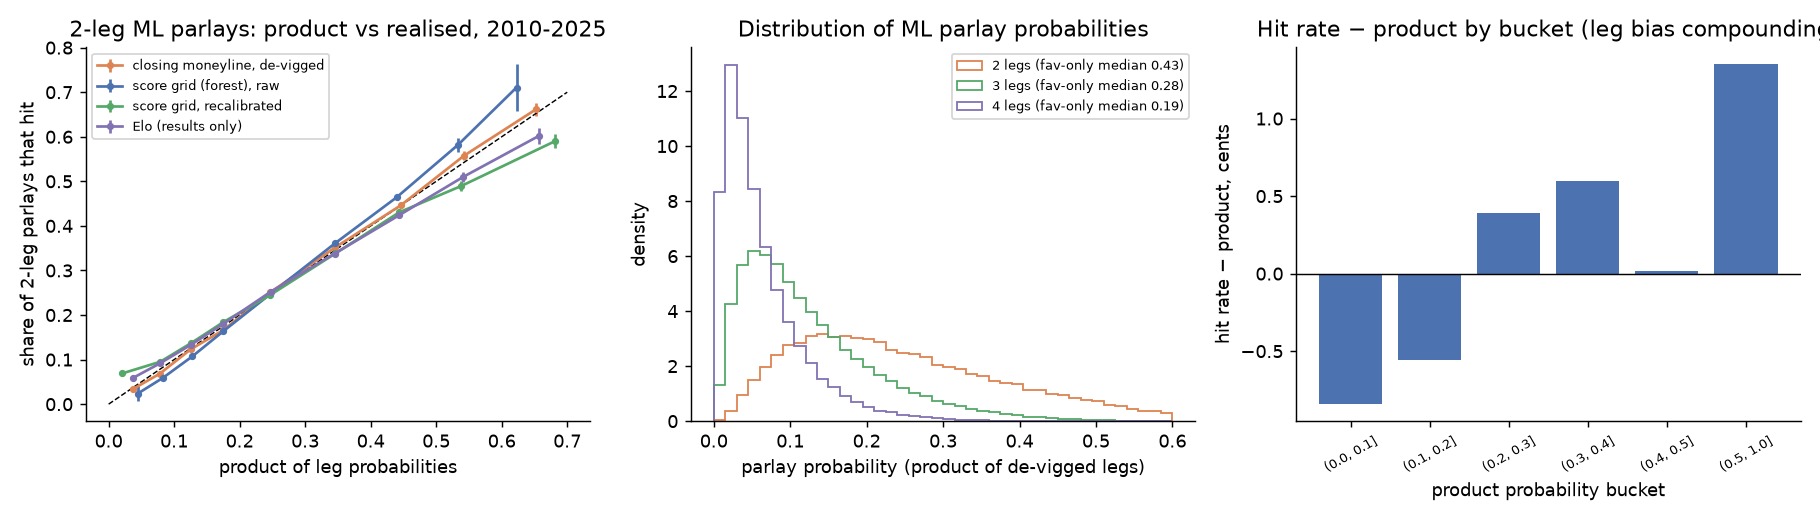
\includegraphics[width=\textwidth]{parlay_ml_history.png}
\caption{Left: share of two-leg parlays that hit against the product of the leg probabilities, by source. Centre: distribution of parlay probabilities by number of legs; the median favourites-only parlay has probability 0.43 (2 legs), 0.28 (3) and 0.18 (4). Right: hit rate minus the book's product, by probability bucket.}
\label{fig:parlay_history}
\end{figure}

Three things come out.
\begin{enumerate}[nosep]
\item \textbf{Multiplying the book's probabilities gives a fair parlay price.} The closing line's product is the most accurate and its slope is 1: a parlay it prices at 40\% hits about 40\% of the time, for favourites and underdogs alike.
\item \textbf{The games are independent.} On the forest's out-of-sample residuals over 2010--2025, the correlation between games on the same date is $-0.005$ (14,426 pairs, standard error 0.008) and between games in the same week $-0.005$; for totals $-0.017$ and $-0.008$. Two home teams in the same week both win 29.5\% of the time against 30.0\% from the product. Multiplication is the right rule across games.
\item \textbf{Our own probabilities are a little less accurate and biased in a known direction.} All three of our sources score about 0.173 against the book's 0.166. More important is how they are wrong: our model gives underdogs too much chance, so a parlay of two favourites that hits 44\% of the time is priced at 37\% by the raw model, and the gap doubles with each leg added. Recalibration halves the gap but does not close it, and Elo, which uses wins alone, behaves the same way. The fix is in the model, not in a correction after the fact: its distribution of margins is too wide for favourites, the same thing the fixed-threshold calibration of Section~\ref{sec:w1021} showed with a slope of 1.2.
\end{enumerate}

\subsubsection{Same-game legs}

Two legs on the same game are not independent, and there the score grid is the model: the parlay's probability is the grid's mass on the intersection of the two legs' regions. Priced on the 2015--2025 grid, the premium over the product of marginals is under half a cent for winner-and-total or spread-and-total combinations (the margin and total of a game are nearly uncorrelated) but 10--25 cents when the legs overlap, such as ``home wins'' with ``home covers $-3$''. We leave same-game parlays for a later report.

\subsubsection{Next steps}

With the Kalshi parlay markets assembled, we will compare each fill with the product of the Kalshi leg mids at the fill hour (the market's own view) and with our model's product, and score all three against settlement. The gap between fill and product tells us what Kalshi charges for a parlay; the gap between our product and the market's tells us where our model disagrees; settlement over several hundred thousand parlays tells us whether those disagreements were worth anything. Before that, we will narrow the model's margin distribution for favourites, since the direction of its error is now known.
